% !TEX root = ../agglo_clust_review.tex


\subsection{Results and discussion}\label{sec:results}
% \subsection{In-depth comparison of different linkage criteria for \algname{}} 
\textbf{Comparison results } Table \ref{tab:results_cremi_train} shows how the agglomerative algorithms derived from our framework compare to each other. For a simple baseline, we also include a segmentation produced by thresholding the affinity predictions (THRESH).
% The poor scores achieved by THRESH highlight the difficulty of the task. 
\algname{} with \emph{Average} linkage, representing one of the new algorithms introduced by our generalized framework, significantly outperformed all other previously proposed agglomerative methods like GAEC (\algname{} Sum), Greedy Fixation (\algname{} Sum + Constraints) or Mutex Watershed (\algname{} Abs. Max.). The competitive performances of this simple parameter-free agglomerative algorithm are also reported by Table \ref{tab:results_cremi_test} that represents the current leader-board of the challenge: all entries, apart from \algname{}, employ superpixel-based post-processing pipelines, several of which rely on the complex multicut problem of \cite{beier2017multicut} that uses several random forests to predict graph edge weights, relying not only on information derived from affinity maps but also raw data and shape information.
Note that the test volumes contain several imaging artifacts that make segmentation particularly challenging and might profit from more robust edge statistics of super-pixel based approaches.
On the other hand, the fact that our algorithm can operate on pixels directly removes the parameter tuning necessary to obtain good super-pixels and can also avoid errors that result from wrong superpixels that cannot be fixed during later agglomeration.
In Appendix \ref{sec:appendix_exps_full_cremi}, we provide more details about how we scaled up \algname{} to the full datasets. Appendix Table \ref{tab:extended_results_cremi} lists the performances and the run-times for all tested \algname{} linkage.


\begin{figure}[t]
        \centering
\begin{minipage}[t]{0.56\textwidth}
% \begin{table}
    \centering
    \scriptsize
    % \begin{subtable}[t!]{0.5\textwidth}\centering
        \begin{tabular}[t]{l|c}
        % \toprule
        % & \multicolumn{2}{c}{\thead{Add Cannot-Link Constraints:}} \\
         % & \multicolumn{1}{c}{\thead{\textsc{No}}} & \multicolumn{1}{c}{\thead{\textsc{Yes}}} \\ \midrule
          & \makecell{CREMI-Score \\(lower is better)} \\ \midrule 
         % & \multicolumn{1}{c}{\thead{$\beta$}}  & \thead{AP} & \multicolumn{1}{c}{\thead{$\beta$}} & \thead{AP} \\ \midrule\midrule
\textbf{Our UNet + \algname{}} \textbf{Average}& \textbf{0.226}  \\
Our UNet + \algname{} Sum + Constraints \cite{levinkov2017comparative} & 0.282 \\
% Our UNet + DTWS + MC & -& 0.310 \\
% Our UNet + DTWS + LMC & -& 0.317 \\
Our UNet + \algname{} Abs. Max. \cite{wolf2018mutex} & 0.322 \\
Our UNet + \algname{} Max. + Constraints & 0.324 \\
Our UNet + \algname{} Sum \cite{keuper2015efficient} & 0.334 \\
Our UNet + \algname{} Average + Constraints & 0.563 \\
Our UNet + THRESH & 1.521 \\ 
Our UNet + \algname{} Min & 2.522 \\
Our UNet + \algname{} Min + Constraints & 2.522 \\
Our UNet + \algname{} Max & 2.626 \\
% \textbf{\algname{}} & \textbf{Average}& \textbf{0.936 $\pm$ 0.004}  \\
% Greedy Fixation \cite{levinkov2017comparative} & Sum + Constr. & 0.906 $\pm$ 0.022 \\
% DTWS + LMC & -& 0.903 $\pm$ 0.016 \\
% DTWS + MC & -& 0.903 $\pm$ 0.017 \\
% % DTWS + avgHC &-& \\
% % DTWS + MC (SR)& -& 0.900 $\pm$ 0.019 \\
% % DTWS + LMC (SR)& -& 0.898 $\pm$ 0.017 \\
% Mutex Watershed \cite{wolf2018mutex} & Abs. Max.  & 0.897 $\pm$ 0.012 \\
% GAEC \cite{keuper2015efficient} & Sum & 0.872 $\pm$ 0.028 \\
% THRESH &-& 0.221  $\pm$ 0.067 \\ 
% % DTWS + \algname{} & Average& \TODO{} \\
% % DTWS  & -& 0.010 $\pm$ 0.003\\
        \end{tabular}
    \captionof{table}{CREMI-Scores achieved by different post-processing methods. Scores are averaged over the three CREMI training datasets}
    \label{tab:results_cremi_train}
\end{minipage}\hfill
\begin{minipage}[t]{0.4\textwidth}
    \centering
    \scriptsize
        \begin{tabular}[t]{l|c}
         & \makecell{CREMI-Score \\(lower is better)}  \\ \midrule
Our UNet + DTWS + LMC &  0.221\\
PNI-UNet \cite{lee2017superhuman} & 0.228 \\
\textbf{Our UNet + \algname{} Average} & \textbf{0.241} \\
MALA-UNet + MC \cite{funke2018large} & 0.276 \\
CRUNet \cite{zeng2017deepem3d} & 0.566  \\
LFC \cite{parag2017anisotropic} & 0.616  \\
% Our UNet + DTWS + LMC &  \textbf{0.221} & \textbf{0.108}\\
% PNI-UNet & 0.228 & 0.116 \\
% Our UNet + \algname{} Avg-Linkage & 0.244 & 0.130 \\
% MALA-UNet + MC \cite{funke2018large} & 0.276 & 0.132 \\
% CRUNet \cite{zeng2017deepem3d} & 0.566 & 0.229 \\
% LFC \cite{parag2017anisotropic} & 0.616 & \\
        \end{tabular}
        \vspace*{4.5em}
    \captionof{table}{Current published entries of the CREMI challenge leaderboard \cite{cremiChallenge} (May 2019) on the three test datasets}
    \label{tab:results_cremi_test}
\end{minipage}
\end{figure}
\captionsetup[subfigure]{justification=centering, singlelinecheck=off}
\begin{figure}
\centering
    %     \begin{subfigure}[t]{0.49 \textwidth}
    %     \centering
    %     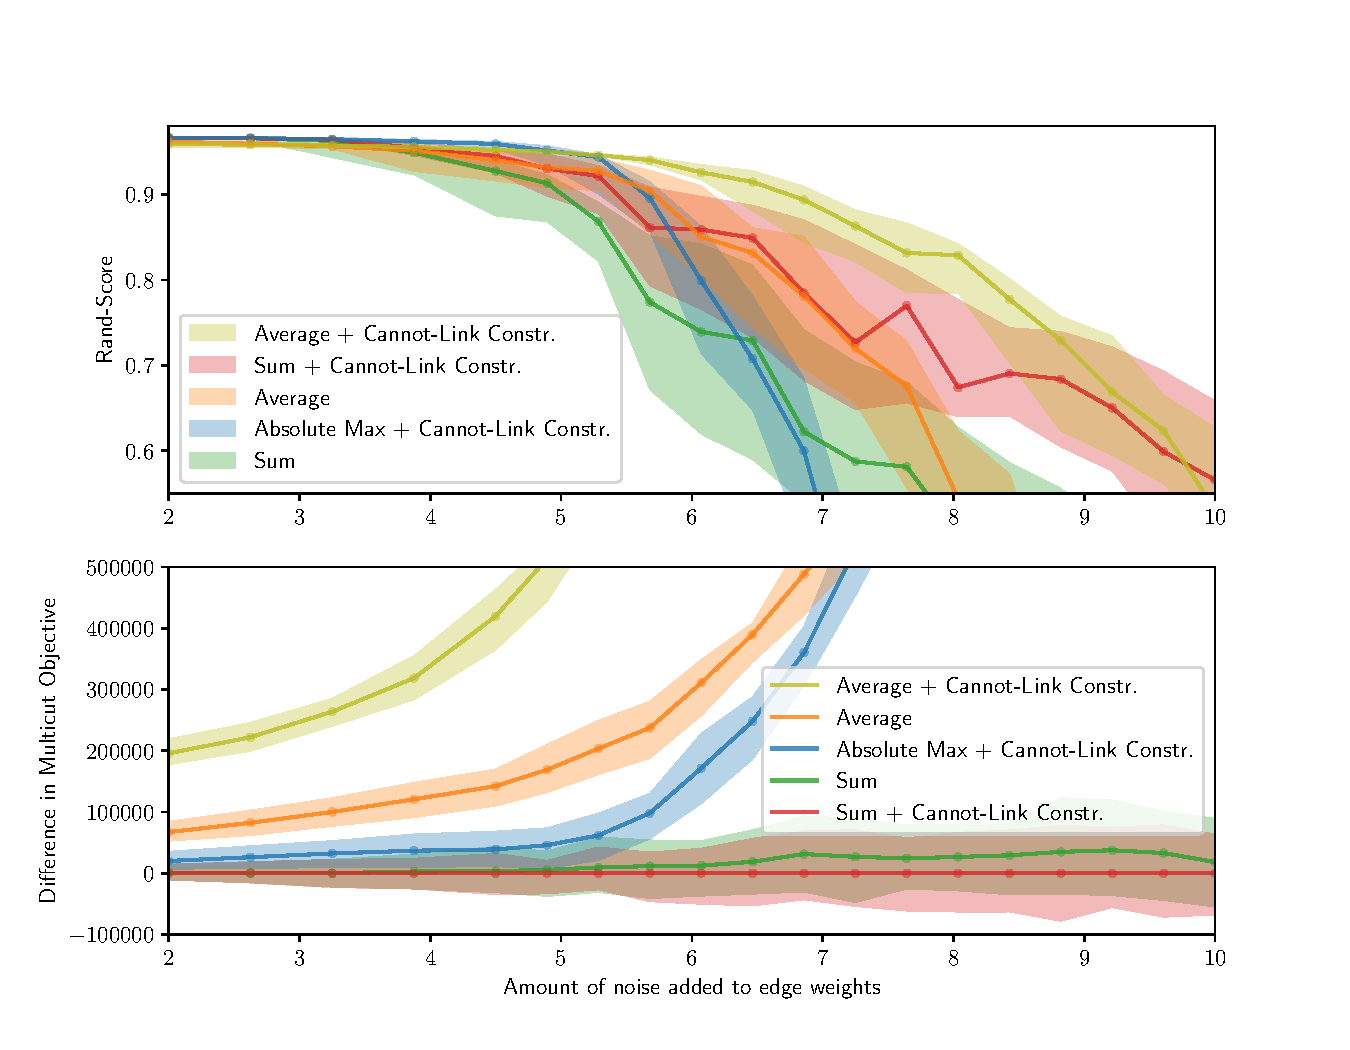
\includegraphics[width=\textwidth,trim=0.55in 0.35in 0.65in 0.80in,clip]{./figs/merge_noise_only_direct.pdf}

    %     \caption{Without long-range edges: $p_{\mathrm{long}}=0$} \label{fig:merge_noise_only_direct}
    % \end{subfigure} \hfill
    % \begin{subfigure}[t]{0.49 \textwidth}
    %     \centering
    %     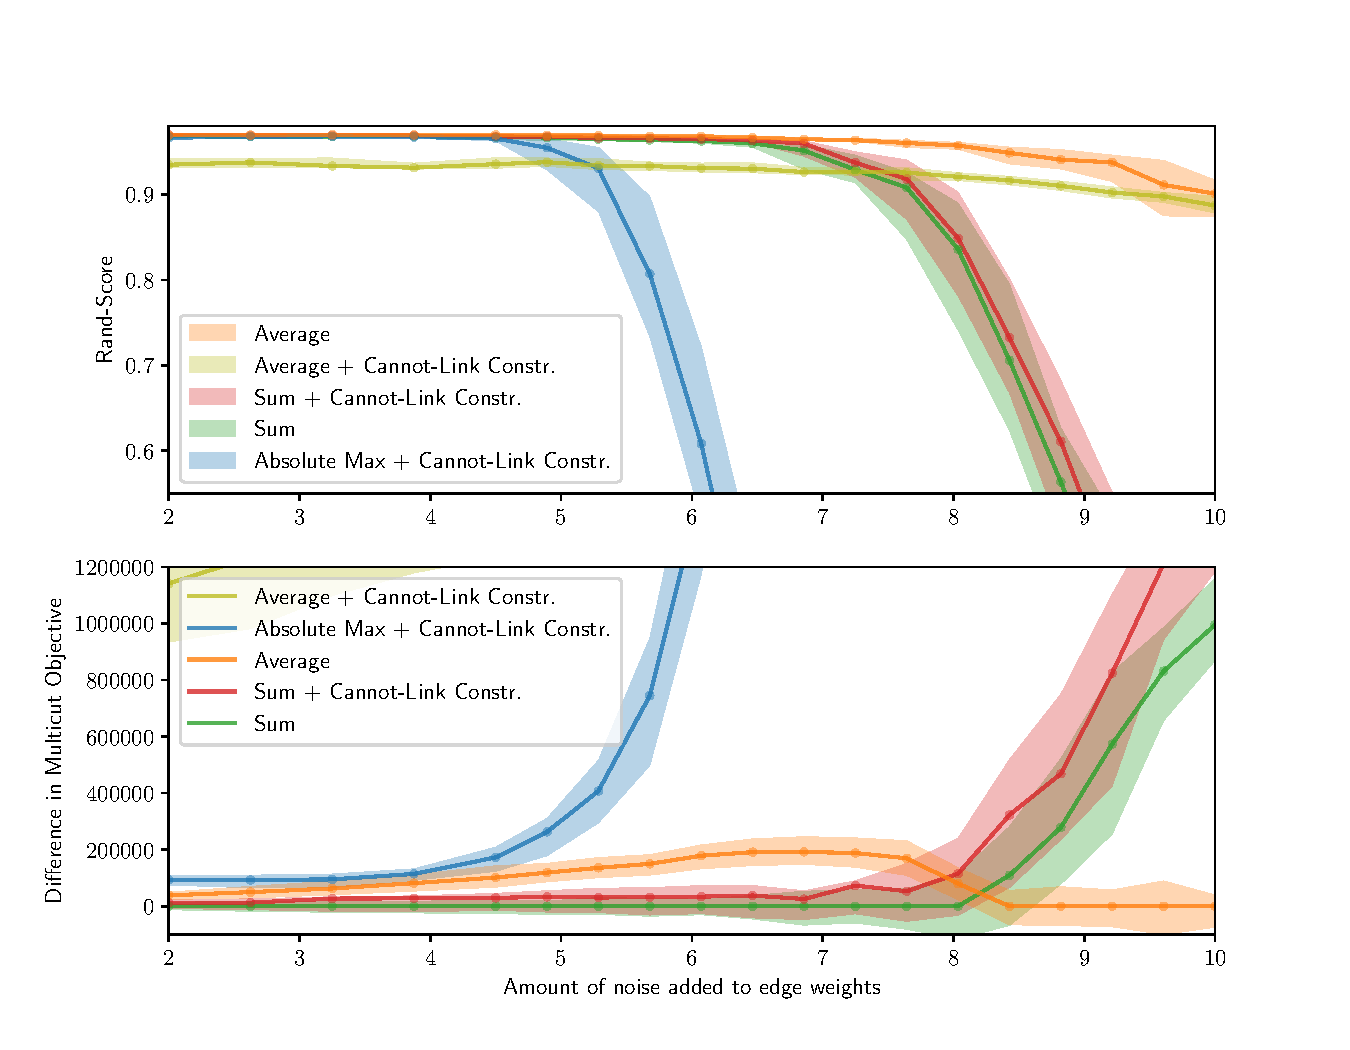
\includegraphics[width=\textwidth,trim=0.53in 0.35in 0.65in 0.80in,clip]{./figs/merge_noise_long_range.pdf}
    %     \caption{With long-range edges: $p_{\mathrm{long}}=0.1$} \label{fig:merge_noise_with_long_range}
    % \end{subfigure}
    \begin{subfigure}[t]{0.49 \textwidth}
        \centering
        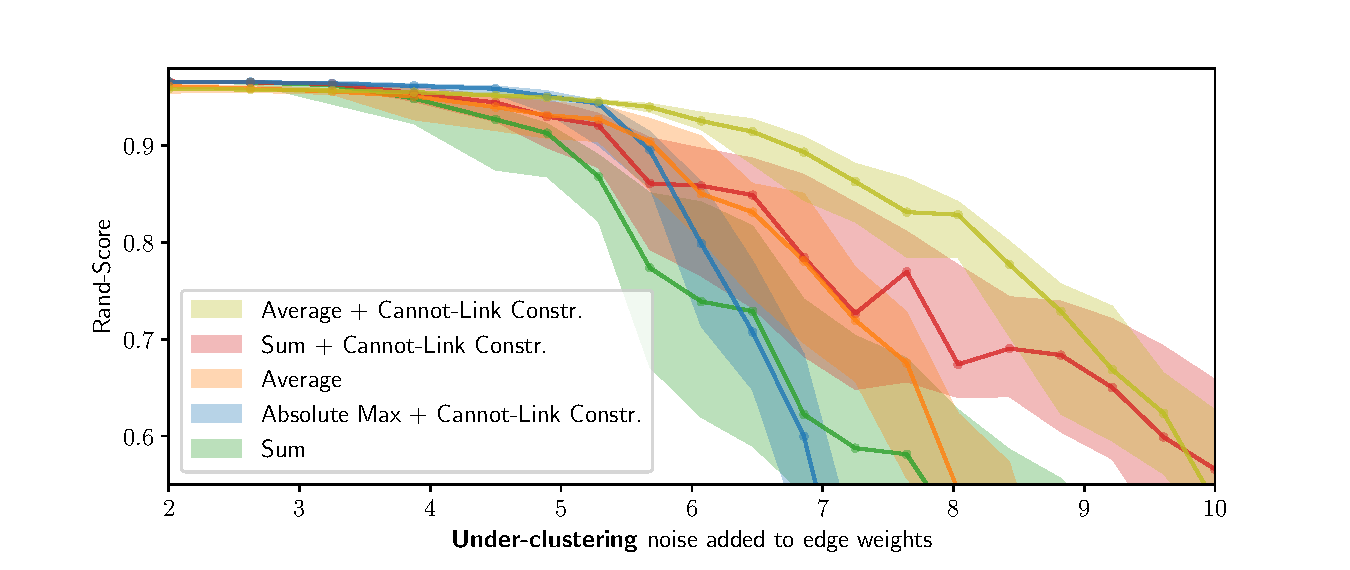
\includegraphics[width=\textwidth,trim=0.55in 0.1in 0.65in 0.45in,clip]{./figs/noise_plots/under_segment_plots_0.pdf}
        % \caption{Without long-range edges: $p_{\mathrm{long}}=0$} \label{fig:merge_noise_only_direct}
    \end{subfigure} \hfill
    \begin{subfigure}[t]{0.49 \textwidth}
        \centering
        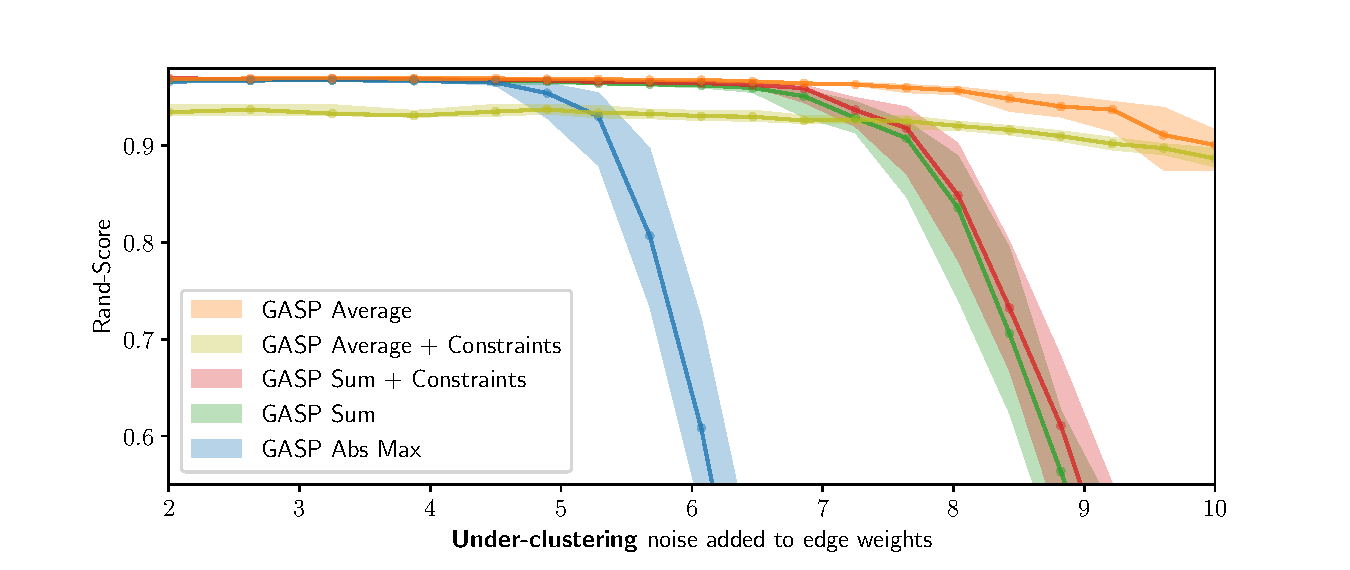
\includegraphics[width=\textwidth,trim=0.53in 0.1in 0.65in 0.45in,clip]{./figs/noise_plots/under_segment_plots_1.pdf}
        % \caption{With long-range edges: $p_{\mathrm{long}}=0.1$} \label{fig:merge_noise_with_long_range}
    \end{subfigure}

        \begin{subfigure}[t]{0.49 \textwidth}
        \centering
        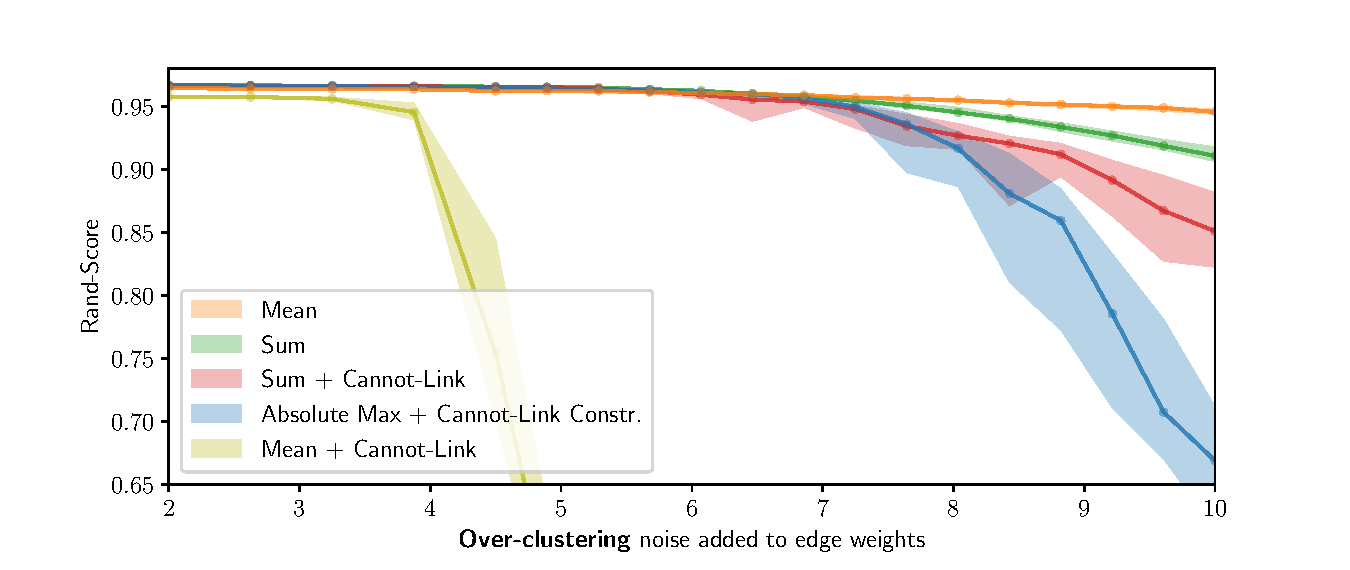
\includegraphics[width=\textwidth,trim=0.53in 0.1in 0.65in 0.45in,clip]{./figs/noise_plots/over_segment_plots_0.pdf}
        \caption{No long-range predictions: $p_{\mathrm{long}}=0$} \label{fig:merge_noise_only_direct}
    \end{subfigure} \hfill
    \begin{subfigure}[t]{0.49 \textwidth}
        \centering
        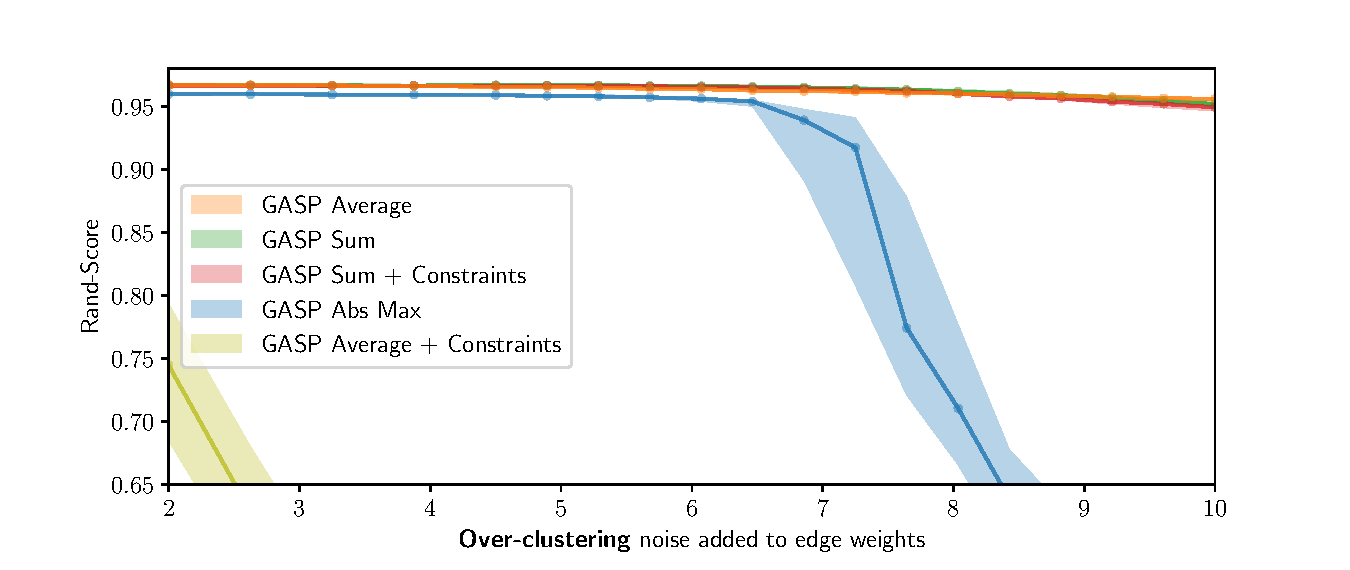
\includegraphics[width=\textwidth,trim=0.53in 0.1in 0.65in 0.45in,clip]{./figs/noise_plots/over_segment_plots_1.pdf}
        \caption{With long-range predictions: $p_{\mathrm{long}}=0.1$} \label{fig:merge_noise_with_long_range}
    \end{subfigure}
\caption{\algname{} sensitivity to noise: \emph{Average} linkage proved to be the most robust. Performances are given by Rand-Score (higher is better) depending on the amount of noise added to the CNN predictions.  Solid lines represent median values over 30 experiments. Values between the 25th and the 75th percentile are shown in shade areas. The two set of experiments using under- and over-clustering noise are summarized in the plots at the top and at the bottom, respectively (see Appendix \ref{sec:appendix_noise_gen} for more details). For each experiment, some of the long-range CNN predictions were randomly selected with probability $p_{\mathrm{long}}$ and added as long-range edges in the pixel grid-graph.
%\textbf{Bottom}: Multicut objective (Eq. \ref{eq:multicut_obj}), measuring how balanced the final clusterings are (lower is better); for a clearer comparison, an offset is added to the energy values, so that the method achieving the lowest energy is always assigned to value zero. 
}\label{fig:noise_plots}
\end{figure}
% \begin{minipage}[b]{0.48\textwidth}
% % \begin{figure}
%         % \begin{subfigure}[t]{0.48 \textwidth}
%         \centering
%         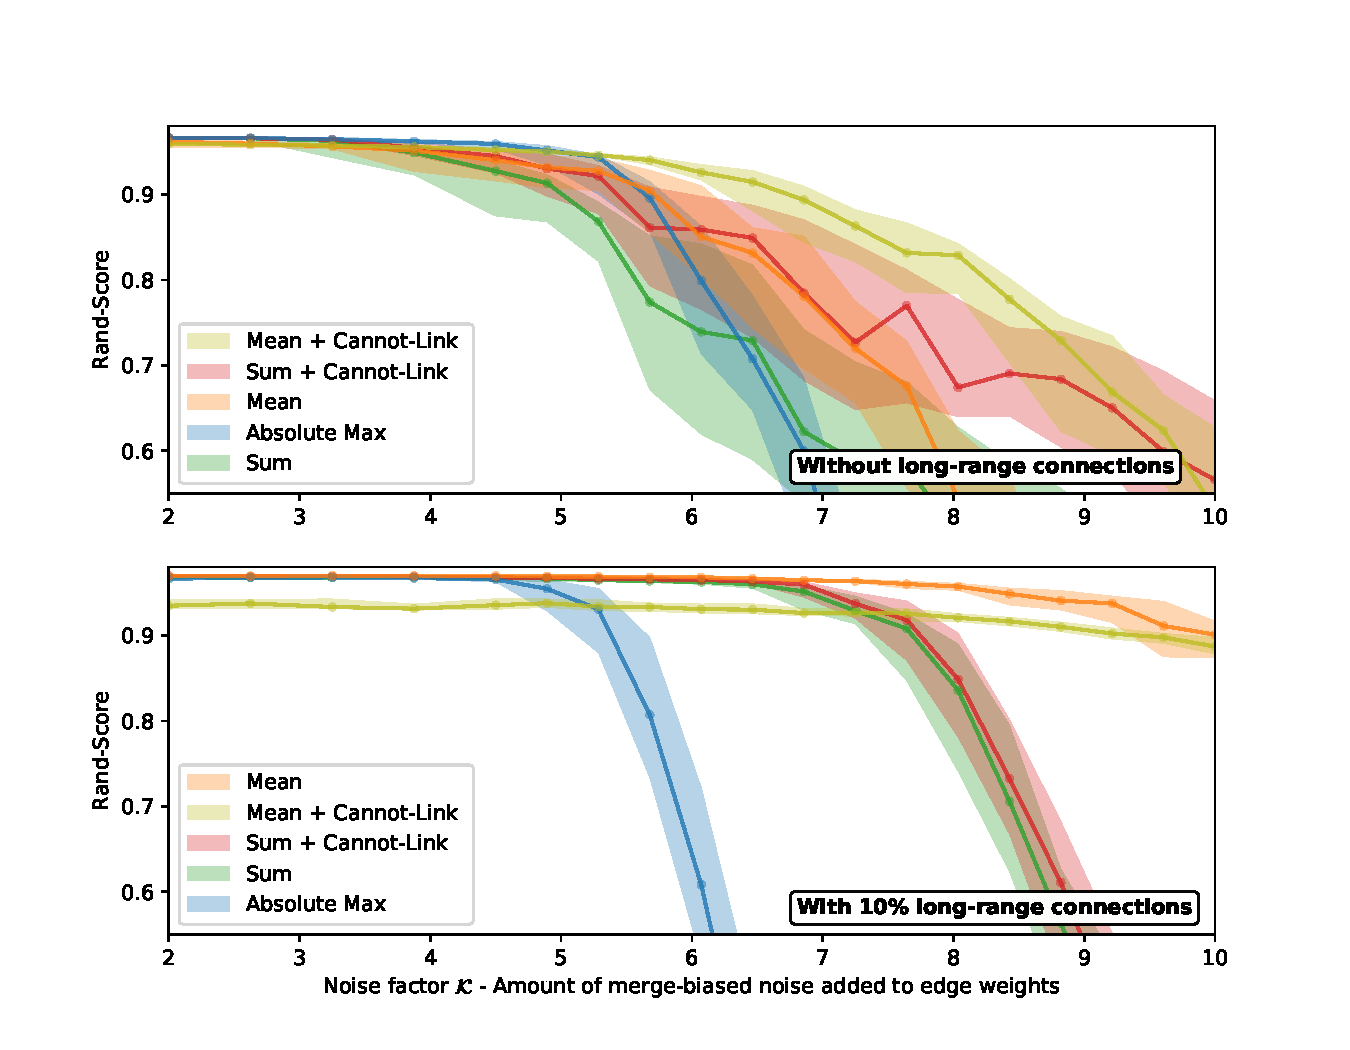
\includegraphics[width=0.98\textwidth,trim=0.35in 0.35in 0.35in 0.35in,clip]{./figs/merge_noise.pdf}
%         \captionof{subfigure}{Merge-biased opensimplex noise} \label{fig:thresh}
%     \end{minipage}\hfil
% \begin{minipage}[b]{0.48\textwidth}
%     % \end{subfigure}%
%     % \begin{subfigure}[t]{0.48 \textwidth}
%         \centering
%         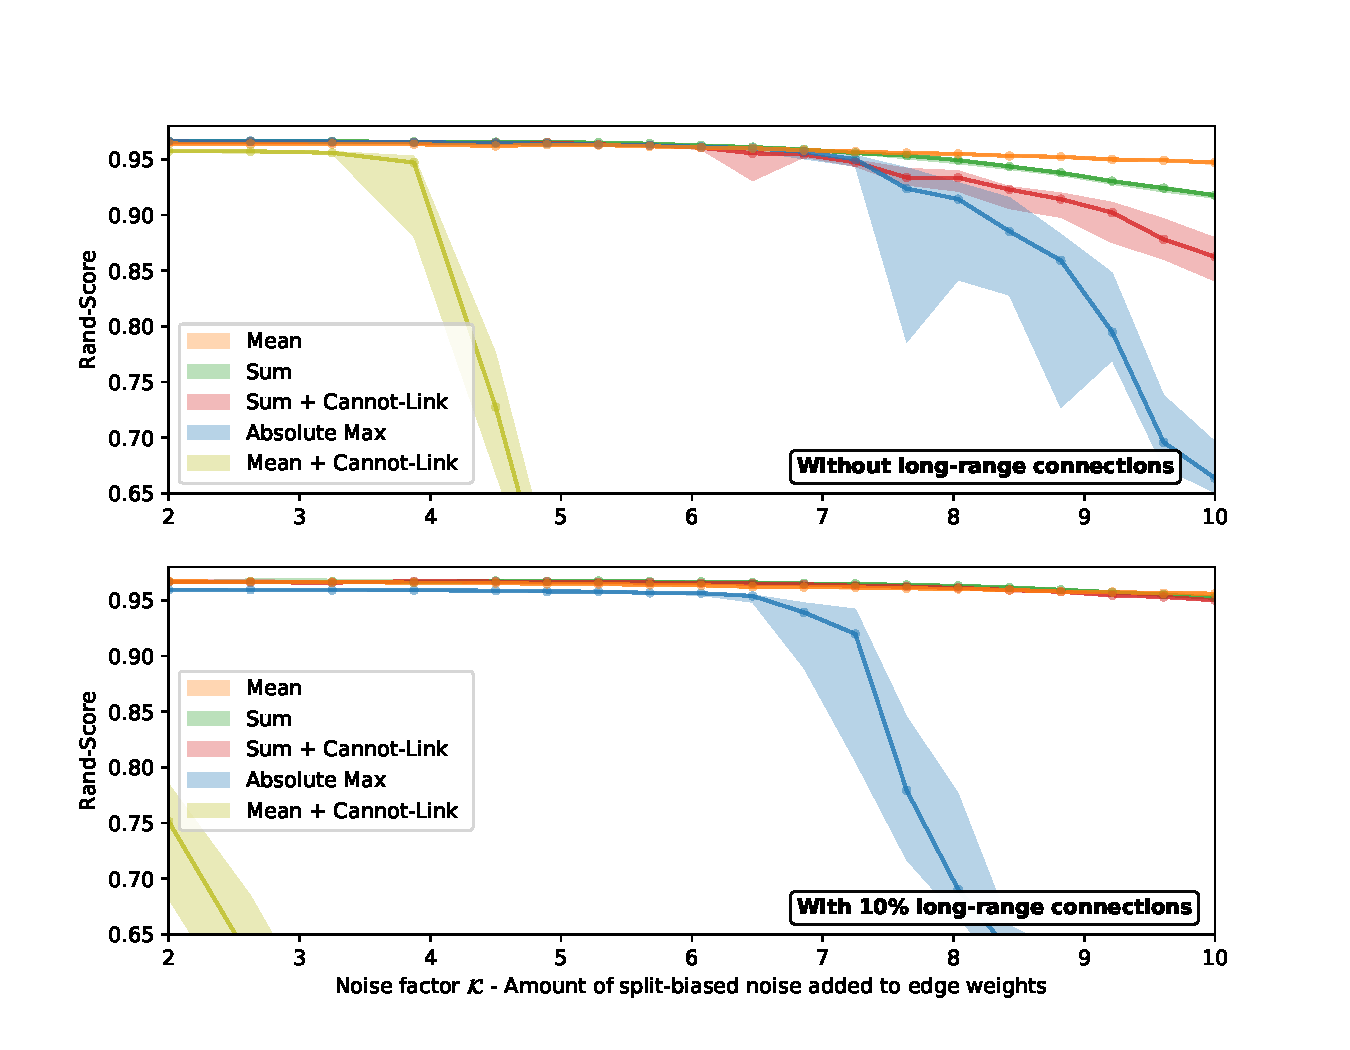
\includegraphics[width=0.98\textwidth,trim=0.29in 0.31in 0.31in 0.31in,clip]{./figs/split_noise.pdf}
%         \captionof{subfigure}{Split-biased opensimplex noise} \label{fig:ws}
%     % \end{subfigure}
% \captionof{figure}{Plot illustrating Adapted RAND scores achieved by UGACA and different update rules when noise is added to the edge weights... Solid lines represent median values, whereas values between the 25th and the 75th percentile are shown in shade areas.    \TODO{Label which uses only local-neighbors and which uses long-range connections}}\label{fig:noise_plots}
% % \end{figure}


\textbf{Noise experiments }  Additionally, we run a set of experiments where the CNN predictions are perturbed by noise, in order to highlight the properties of each \algname{} algorithm and perform an in-depth comparison that is as quantitative as possible. Appendix \ref{sec:appendix_noise_gen} introduces the type of spatially correlated noise that allowed us to perturb the CNN outputs by introducing simulated additional artifacts like missing or false boundary evidences.  
Fig. \ref{fig:noise_plots} summarize our 12000 noise experiments: we focus on the best performing linkage criteria, i.e. \emph{Average}, \emph{Sum} and \emph{Abs Max}, and test them with different values of noise. 
In these experiments, we also want to assess how beneficial it is to use long-range CNN predictions in the agglomeration. Thus, we perform a set of simulations without adding long-range connections to the grid-graph and another set where we introduce them with a 10\% probability\footnote{We also performed experiments adding all the long-range predictions given by the CNN model, but we did not note major differences with the case using only 10\% of them. Adding this small portion is usually sufficient to improve the scores.}.
%, both with and without use of long-range connections in the grid-graph. % In Fig. \ref{fig:noise_plots}, we used a merge-biased noise decreasing boundary evidence. See Fig. \ref{fig:noise_split} in Appendix for a split-biased version. 

\textbf{Average and Abs Max linkage } Our findings confirm that \algname{} with \emph{Average} linkage criterion represents the most robust algorithm tested and the one that benefits the most from using the long-range CNN predictions. On the other hand, it is not a surprise that the \emph{Abs Max} statistic proposed by \cite{wolf2018mutex} is less robust to noise than the \emph{Average} linkage, but, as we show in the Appendix Table \ref{tab:extended_results_cremi}, \emph{Abs Max} represents a valid and considerably faster option. 
Adding long-range connections to the graph is generally helpful, but when many of them carry repulsive weights, then \algname{} with cannot-link constraints shows a clear tendency to over-cluster.    

\textbf{Sum linkage } 
% The \emph{Sum} linkage generally outputs the most balanced graph partitioning according to the objective defined in Eq. \ref{eq:multicut_obj} and is then confirmed to be a good choice for initializing more complex approximations of the multicut optimization problem like \cite{beier2016efficient}. 
All our experiments show that \algname{} with \emph{Sum} linkage is the algorithm with the highest tendency to under-cluster and incorrectly merge segments (see Fig. \ref{fig:cremi_comparison} for an example). This property is related to the empirical observation that a \emph{Sum} statistic tends to grow clusters one after the other, as shown in Fig. \ref{fig:intro_figure} by the quite unique agglomeration order of the \emph{Sum} statistic. An intuitive explanation of this fact is the following: initially, most of the intra-cluster nodes present similar attractive interactions between each others; when the two nodes sharing the most attractive interaction are merged, there is a high chance that they both share an attractive interaction with a common neighboring node, so the new interaction with this common neighbor will be immediately assigned to a high priority in the agglomeration, given by the sum of two high weights; this usually starts a ``chain reaction'', where only a single cluster is agglomerated at the beginning. On the other hand, as we also see in Fig. \ref{fig:intro_figure}, other linkage criteria like \emph{Average} or \emph{Abs Max} grow clusters of similar sizes in parallel and accumulate in this way much more reliable inter-cluster statistics.





